%
% Roadmap - The way forward
%

\part{Roadmap -- The way forward}\index{Roadmap}\label{part:roadmap}

\famousquote{You got to go down a lot of wrong roads to find the right one.}{Bob Parsons}
\newline

\famousquote{The further a society drifts from the truth, the more it will hate those that speak it.}{George Orwell}

\section{The tech-web for the quantum future}

\dropcap{W}{e} have in this work presented a vast number of ideas, protocols, applications and implications for future quantum technology, mediated by the quantum internet. The relationship between all these concepts is highly complex, with a large number of interdependencies. In Fig.~\ref{fig:roadmap} we express this as a mind-map timeline\index{Mind-map}\index{Timelines}, capturing these relationships to show the logical flow of developments that will need to take place to reach various technological milestones and destinations.

Note that the evolution of future quantum technologies proceeds as a \textit{tech-web}\index{Tech-web} rather than as a strictly linear progression. This necessitates that many quantum technology research projects will need to execute in parallel to achieve multiple desired endpoints in a timely manner without bottlenecks.

\begin{figure*}
	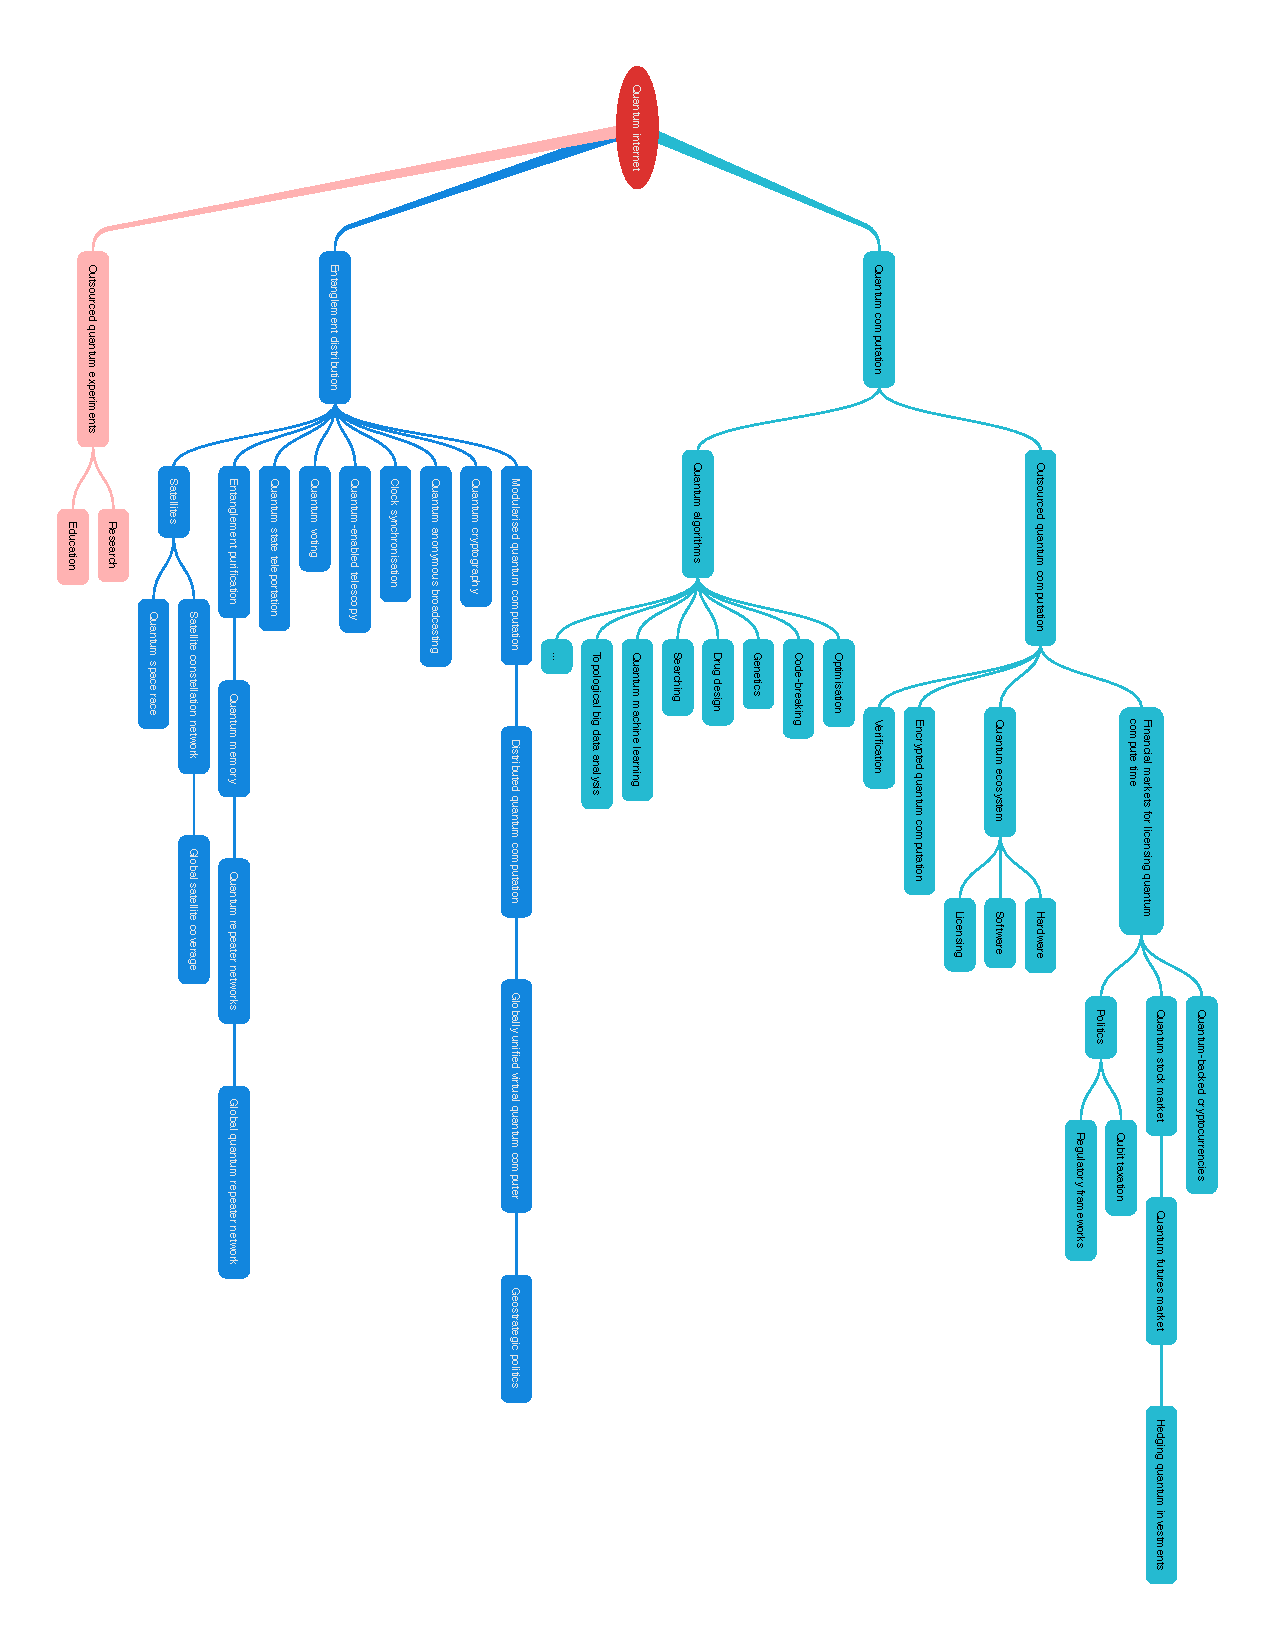
\includegraphics[clip=true, angle=-90, width=\textwidth]{roadmap}
	\caption{Relationships and dependencies in the development and deployment of the major concepts in the quantum internet -- the quantum \textit{tech-web}\index{Tech-web} -- showing the logical flow of developments that will need to take place to reach various technological milestones and destinations. The progression is highly non-linear, mandating many research programs operating in parallel to prevent technology bottlenecks.}\label{fig:roadmap}
\end{figure*}
